% Entorno empresarial.
\chapter{Entorno Empresarial} \label{chap:Entorno Empresarial}

\vspace{5 mm}


En esta sección se describe el ambiente organizacional en el que se desarrolló el proyecto de pasantía de la aplicación web y móvil de \textit{Notificaciones+}. Se presenta la empresa Synergy-GB, sus valores, objetivos y estructura organizativa.


Synergy-GB es una empresa perteneciente al grupo Corporativo SYNERGY-GB Corporation, dedicada al desarrollo y comercialización de productos bajo Tecnologías de Información. Estudia las tendencias a nivel de aplicaciones corporativas actuales a las empresas, a fin de ofrecer soluciones en sus mercados que estén en línea con las prioridades gerenciales y de negocio del mundo actual.

La cartera de aplicaciones va desde Soluciones Integrales Sistémicas que resuelven una problemática compleja en la empresa, hasta Soluciones Puntuales Departamentales que resuelven problemas específicos en procesos de negocio donde se ha perdido el control gerencial  \cite{ESGB0}.


La misión de la empresa, según revela su portal web es “crear, desarrollar y apoyar modelos de negocio que mejoren la competitividad y productividad de sus clientes”  \cite{ESGB0}. 
La visión de Synergy-GB es “Convertir a Synergy-GB en una organización de alcance hispanoamericano, que combine en forma creativa, ideas, talento, tecnología, visión empresarial, innovación y excelencia en el servicio”  \cite{ESGB0}. 
Los valores que definen a Synergy-GB como empresa son \cite{ESGB0}:
\begin{itemize}[noitemsep,nolistsep]
\item Compromiso con la Calidad.
\item Compromiso con la Satisfacción al Cliente.
\item Compromiso con la Generación de un Legado.
\item Sentido de Propiedad.
\item Sentido Emprendedor.
\item Integridad y Honestidad.
\item Orientación a Resultados.
\item Compromiso con la Innovación y el Desarrollo de nuevas ideas.
\item Proactividad.
\item Trabajo en Equipo.
\item Socialmente Responsables.
\item Comercialmente Astutos.
\item Diversión como elemento catalizador.
\end{itemize}

En la Figura ~\ref{fig:estsyn} se presenta la estructura organizativa de la empresa \cite{ESGB1}. El desarrollador ocupó el puesto de pasante en el área de aplicaciones.

\begin{figure}[ht]
  \centering
  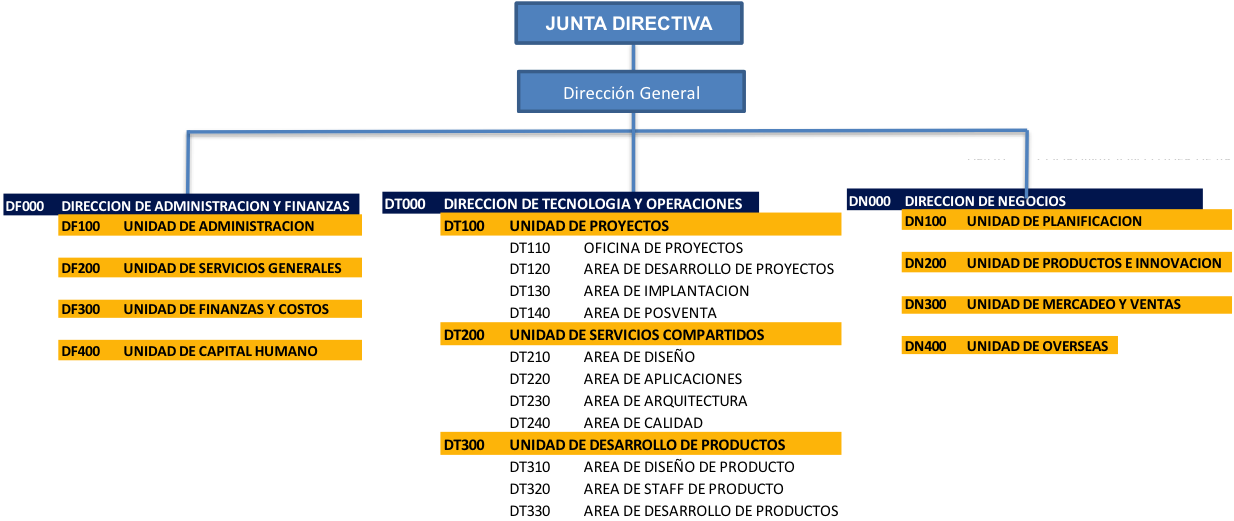
\includegraphics[scale=0.6,type=png,ext=.png,read=.png,angle=0,origin=c]{imagenes/estructurasynergy}
  \caption{Estructura Organizativa de Synergy-GB, C.A.}
  \label{fig:estsyn}
\end{figure}


Entre las áreas de la empresa, las siguientes son las más relevantes \cite{ESGB2}:
\begin{itemize}[noitemsep,nolistsep]
\item {Oficina de proyectos:} 

Se ocupa de centralizar y coordinar la dirección de proyectos. 

\item {Diseño e Imagen:}

Encargada de realizar los diseños que proyecten la imagen Corporativa de la empresa y además de los diseños adecuados a la imagen de cada cliente de acuerdo a los objetivos de cada proyecto. 

\item {Posventa:}

Gestiona la relación con los clientes después que se implantan las soluciones, productos o servicios que ofrece la empresa, además se encarga de gestionar la atención de incidencias, errores, fallas, reclamos, mantenimiento, actualizaciones o requerimientos de nuestros clientes. 
 
\item {Calidad e Implantación:}
 
Se encarga de velar por la calidad de los servicios que ofrece la empresa de forma integral, desde los procesos, la metodología de trabajo y ejecución de proyectos hasta las encuestas de satisfacción después que se entrega una solución.

\item {Administración:}

Gerencia los procesos relacionados con la gestión de la información financiera y laboral de la empresa.

\item {Aplicaciones:}

Se encarga de gerenciar la fábrica de proyectos y productos en particular, la asignación del Talento a los diversos proyectos, productos o servicios de fábrica, implantación o posventa. El área desarrolla los Skills técnicos para el desarrollo de aplicaciones Móviles o Web así como la Integración de plataformas con foco continuo en la Innovación tecnológica y la entrega de soluciones de vanguardia.

\item {Unidad Comercial:}

Es la encargada de la gestión de ventas y relacionamiento con clientes y prospectos, coordinando las actividades que permitan llevar una oportunidad desde su detección (proactiva o reactivamente), hasta la presentación y negociación del cierre de la misma en el marco de una metodología que garantice una alta probabilidad de éxito.  

\item {Unidad Productos:} 

Es la máxima responsable de la gestión de productos de la organización. Su responsabilidad abarca desde la concepción de los productos hasta su maduración y consolidación. Gestiona los productos a lo largo de todo su ciclo de vida ayudando en cada momento a definir las estrategias comerciales y de mercadeo a seguir. 



\end{itemize}
